% Options for packages loaded elsewhere
\PassOptionsToPackage{unicode}{hyperref}
\PassOptionsToPackage{hyphens}{url}
\PassOptionsToPackage{dvipsnames,svgnames,x11names}{xcolor}
%
\documentclass[
  10pt,
  a5paper,
  DIV=11,
  numbers=noendperiod]{scrreprt}

\usepackage{amsmath,amssymb}
\usepackage{iftex}
\ifPDFTeX
  \usepackage[T1]{fontenc}
  \usepackage[utf8]{inputenc}
  \usepackage{textcomp} % provide euro and other symbols
\else % if luatex or xetex
  \usepackage{unicode-math}
  \defaultfontfeatures{Scale=MatchLowercase}
  \defaultfontfeatures[\rmfamily]{Ligatures=TeX,Scale=1}
\fi
\usepackage{lmodern}
\ifPDFTeX\else  
    % xetex/luatex font selection
    \setmainfont[]{Cambria}
    \setsansfont[]{Corbel}
    \setmonofont[]{Consolas}
\fi
% Use upquote if available, for straight quotes in verbatim environments
\IfFileExists{upquote.sty}{\usepackage{upquote}}{}
\IfFileExists{microtype.sty}{% use microtype if available
  \usepackage[]{microtype}
  \UseMicrotypeSet[protrusion]{basicmath} % disable protrusion for tt fonts
}{}
\makeatletter
\@ifundefined{KOMAClassName}{% if non-KOMA class
  \IfFileExists{parskip.sty}{%
    \usepackage{parskip}
  }{% else
    \setlength{\parindent}{0pt}
    \setlength{\parskip}{6pt plus 2pt minus 1pt}}
}{% if KOMA class
  \KOMAoptions{parskip=half}}
\makeatother
\usepackage{xcolor}
\setlength{\emergencystretch}{3em} % prevent overfull lines
\setcounter{secnumdepth}{5}
% Make \paragraph and \subparagraph free-standing
\makeatletter
\ifx\paragraph\undefined\else
  \let\oldparagraph\paragraph
  \renewcommand{\paragraph}{
    \@ifstar
      \xxxParagraphStar
      \xxxParagraphNoStar
  }
  \newcommand{\xxxParagraphStar}[1]{\oldparagraph*{#1}\mbox{}}
  \newcommand{\xxxParagraphNoStar}[1]{\oldparagraph{#1}\mbox{}}
\fi
\ifx\subparagraph\undefined\else
  \let\oldsubparagraph\subparagraph
  \renewcommand{\subparagraph}{
    \@ifstar
      \xxxSubParagraphStar
      \xxxSubParagraphNoStar
  }
  \newcommand{\xxxSubParagraphStar}[1]{\oldsubparagraph*{#1}\mbox{}}
  \newcommand{\xxxSubParagraphNoStar}[1]{\oldsubparagraph{#1}\mbox{}}
\fi
\makeatother

\usepackage{color}
\usepackage{fancyvrb}
\newcommand{\VerbBar}{|}
\newcommand{\VERB}{\Verb[commandchars=\\\{\}]}
\DefineVerbatimEnvironment{Highlighting}{Verbatim}{commandchars=\\\{\}}
% Add ',fontsize=\small' for more characters per line
\usepackage{framed}
\definecolor{shadecolor}{RGB}{241,243,245}
\newenvironment{Shaded}{\begin{snugshade}}{\end{snugshade}}
\newcommand{\AlertTok}[1]{\textcolor[rgb]{0.68,0.00,0.00}{#1}}
\newcommand{\AnnotationTok}[1]{\textcolor[rgb]{0.37,0.37,0.37}{#1}}
\newcommand{\AttributeTok}[1]{\textcolor[rgb]{0.40,0.45,0.13}{#1}}
\newcommand{\BaseNTok}[1]{\textcolor[rgb]{0.68,0.00,0.00}{#1}}
\newcommand{\BuiltInTok}[1]{\textcolor[rgb]{0.00,0.23,0.31}{#1}}
\newcommand{\CharTok}[1]{\textcolor[rgb]{0.13,0.47,0.30}{#1}}
\newcommand{\CommentTok}[1]{\textcolor[rgb]{0.37,0.37,0.37}{#1}}
\newcommand{\CommentVarTok}[1]{\textcolor[rgb]{0.37,0.37,0.37}{\textit{#1}}}
\newcommand{\ConstantTok}[1]{\textcolor[rgb]{0.56,0.35,0.01}{#1}}
\newcommand{\ControlFlowTok}[1]{\textcolor[rgb]{0.00,0.23,0.31}{\textbf{#1}}}
\newcommand{\DataTypeTok}[1]{\textcolor[rgb]{0.68,0.00,0.00}{#1}}
\newcommand{\DecValTok}[1]{\textcolor[rgb]{0.68,0.00,0.00}{#1}}
\newcommand{\DocumentationTok}[1]{\textcolor[rgb]{0.37,0.37,0.37}{\textit{#1}}}
\newcommand{\ErrorTok}[1]{\textcolor[rgb]{0.68,0.00,0.00}{#1}}
\newcommand{\ExtensionTok}[1]{\textcolor[rgb]{0.00,0.23,0.31}{#1}}
\newcommand{\FloatTok}[1]{\textcolor[rgb]{0.68,0.00,0.00}{#1}}
\newcommand{\FunctionTok}[1]{\textcolor[rgb]{0.28,0.35,0.67}{#1}}
\newcommand{\ImportTok}[1]{\textcolor[rgb]{0.00,0.46,0.62}{#1}}
\newcommand{\InformationTok}[1]{\textcolor[rgb]{0.37,0.37,0.37}{#1}}
\newcommand{\KeywordTok}[1]{\textcolor[rgb]{0.00,0.23,0.31}{\textbf{#1}}}
\newcommand{\NormalTok}[1]{\textcolor[rgb]{0.00,0.23,0.31}{#1}}
\newcommand{\OperatorTok}[1]{\textcolor[rgb]{0.37,0.37,0.37}{#1}}
\newcommand{\OtherTok}[1]{\textcolor[rgb]{0.00,0.23,0.31}{#1}}
\newcommand{\PreprocessorTok}[1]{\textcolor[rgb]{0.68,0.00,0.00}{#1}}
\newcommand{\RegionMarkerTok}[1]{\textcolor[rgb]{0.00,0.23,0.31}{#1}}
\newcommand{\SpecialCharTok}[1]{\textcolor[rgb]{0.37,0.37,0.37}{#1}}
\newcommand{\SpecialStringTok}[1]{\textcolor[rgb]{0.13,0.47,0.30}{#1}}
\newcommand{\StringTok}[1]{\textcolor[rgb]{0.13,0.47,0.30}{#1}}
\newcommand{\VariableTok}[1]{\textcolor[rgb]{0.07,0.07,0.07}{#1}}
\newcommand{\VerbatimStringTok}[1]{\textcolor[rgb]{0.13,0.47,0.30}{#1}}
\newcommand{\WarningTok}[1]{\textcolor[rgb]{0.37,0.37,0.37}{\textit{#1}}}

\providecommand{\tightlist}{%
  \setlength{\itemsep}{0pt}\setlength{\parskip}{0pt}}\usepackage{longtable,booktabs,array}
\usepackage{calc} % for calculating minipage widths
% Correct order of tables after \paragraph or \subparagraph
\usepackage{etoolbox}
\makeatletter
\patchcmd\longtable{\par}{\if@noskipsec\mbox{}\fi\par}{}{}
\makeatother
% Allow footnotes in longtable head/foot
\IfFileExists{footnotehyper.sty}{\usepackage{footnotehyper}}{\usepackage{footnote}}
\makesavenoteenv{longtable}
\usepackage{graphicx}
\makeatletter
\def\maxwidth{\ifdim\Gin@nat@width>\linewidth\linewidth\else\Gin@nat@width\fi}
\def\maxheight{\ifdim\Gin@nat@height>\textheight\textheight\else\Gin@nat@height\fi}
\makeatother
% Scale images if necessary, so that they will not overflow the page
% margins by default, and it is still possible to overwrite the defaults
% using explicit options in \includegraphics[width, height, ...]{}
\setkeys{Gin}{width=\maxwidth,height=\maxheight,keepaspectratio}
% Set default figure placement to htbp
\makeatletter
\def\fps@figure{htbp}
\makeatother
% definitions for citeproc citations
\NewDocumentCommand\citeproctext{}{}
\NewDocumentCommand\citeproc{mm}{%
  \begingroup\def\citeproctext{#2}\cite{#1}\endgroup}
\makeatletter
 % allow citations to break across lines
 \let\@cite@ofmt\@firstofone
 % avoid brackets around text for \cite:
 \def\@biblabel#1{}
 \def\@cite#1#2{{#1\if@tempswa , #2\fi}}
\makeatother
\newlength{\cslhangindent}
\setlength{\cslhangindent}{1.5em}
\newlength{\csllabelwidth}
\setlength{\csllabelwidth}{3em}
\newenvironment{CSLReferences}[2] % #1 hanging-indent, #2 entry-spacing
 {\begin{list}{}{%
  \setlength{\itemindent}{0pt}
  \setlength{\leftmargin}{0pt}
  \setlength{\parsep}{0pt}
  % turn on hanging indent if param 1 is 1
  \ifodd #1
   \setlength{\leftmargin}{\cslhangindent}
   \setlength{\itemindent}{-1\cslhangindent}
  \fi
  % set entry spacing
  \setlength{\itemsep}{#2\baselineskip}}}
 {\end{list}}
\usepackage{calc}
\newcommand{\CSLBlock}[1]{\hfill\break\parbox[t]{\linewidth}{\strut\ignorespaces#1\strut}}
\newcommand{\CSLLeftMargin}[1]{\parbox[t]{\csllabelwidth}{\strut#1\strut}}
\newcommand{\CSLRightInline}[1]{\parbox[t]{\linewidth - \csllabelwidth}{\strut#1\strut}}
\newcommand{\CSLIndent}[1]{\hspace{\cslhangindent}#1}

\KOMAoption{captions}{tableheading}
\makeatletter
\@ifpackageloaded{bookmark}{}{\usepackage{bookmark}}
\makeatother
\makeatletter
\@ifpackageloaded{caption}{}{\usepackage{caption}}
\AtBeginDocument{%
\ifdefined\contentsname
  \renewcommand*\contentsname{Table of contents}
\else
  \newcommand\contentsname{Table of contents}
\fi
\ifdefined\listfigurename
  \renewcommand*\listfigurename{List of Figures}
\else
  \newcommand\listfigurename{List of Figures}
\fi
\ifdefined\listtablename
  \renewcommand*\listtablename{List of Tables}
\else
  \newcommand\listtablename{List of Tables}
\fi
\ifdefined\figurename
  \renewcommand*\figurename{Figure}
\else
  \newcommand\figurename{Figure}
\fi
\ifdefined\tablename
  \renewcommand*\tablename{Table}
\else
  \newcommand\tablename{Table}
\fi
}
\@ifpackageloaded{float}{}{\usepackage{float}}
\floatstyle{ruled}
\@ifundefined{c@chapter}{\newfloat{codelisting}{h}{lop}}{\newfloat{codelisting}{h}{lop}[chapter]}
\floatname{codelisting}{Listing}
\newcommand*\listoflistings{\listof{codelisting}{List of Listings}}
\makeatother
\makeatletter
\makeatother
\makeatletter
\@ifpackageloaded{caption}{}{\usepackage{caption}}
\@ifpackageloaded{subcaption}{}{\usepackage{subcaption}}
\makeatother
\ifLuaTeX
\usepackage[bidi=basic]{babel}
\else
\usepackage[bidi=default]{babel}
\fi
\babelprovide[main,import]{ukrainian}
\ifPDFTeX
\else
\babelfont{rm}[]{Cambria}
\fi
% get rid of language-specific shorthands (see #6817):
\let\LanguageShortHands\languageshorthands
\def\languageshorthands#1{}
\ifLuaTeX
  \usepackage{selnolig}  % disable illegal ligatures
\fi
\usepackage{bookmark}

\IfFileExists{xurl.sty}{\usepackage{xurl}}{} % add URL line breaks if available
\urlstyle{same} % disable monospaced font for URLs
\hypersetup{
  pdftitle={Технології політико-психологічних досліджень},
  pdfauthor={Олександр Виноградов},
  pdflang={uk-UA},
  colorlinks=true,
  linkcolor={blue},
  filecolor={Maroon},
  citecolor={Blue},
  urlcolor={Blue},
  pdfcreator={LaTeX via pandoc}}

\title{Технології політико-психологічних досліджень}
\author{Олександр Виноградов}
\date{2024-05-18}

\begin{document}
\maketitle

\renewcommand*\contentsname{Зміст}
{
\hypersetup{linkcolor=}
\setcounter{tocdepth}{2}
\tableofcontents
}
\bookmarksetup{startatroot}

\chapter*{Передмова}\label{ux43fux435ux440ux435ux434ux43cux43eux432ux430}
\addcontentsline{toc}{chapter}{Передмова}

\markboth{Передмова}{Передмова}

\section*{Вступ}\label{ux432ux441ux442ux443ux43f}
\addcontentsline{toc}{section}{Вступ}

\markright{Вступ}

\section*{Розділ І. Якісні методи психологічного
дослідження.}\label{ux440ux43eux437ux434ux456ux43b-ux456.-ux44fux43aux456ux441ux43dux456-ux43cux435ux442ux43eux434ux438-ux43fux441ux438ux445ux43eux43bux43eux433ux456ux447ux43dux43eux433ux43e-ux434ux43eux441ux43bux456ux434ux436ux435ux43dux43dux44f.}
\addcontentsline{toc}{section}{Розділ І. Якісні методи психологічного
дослідження.}

\markright{Розділ І. Якісні методи психологічного дослідження.}

\subsection*{1.1.
Фокус--групи}\label{ux444ux43eux43aux443ux441ux433ux440ux443ux43fux438}
\addcontentsline{toc}{subsection}{1.1. Фокус--групи}

\subsection*{1.2. Глибинне
інтерв'ю}\label{ux433ux43bux438ux431ux438ux43dux43dux435-ux456ux43dux442ux435ux440ux432ux44e}
\addcontentsline{toc}{subsection}{1.2. Глибинне інтерв'ю}

\section*{Розділ ІІ. Кількісні методи психологічного
дослідження.}\label{ux440ux43eux437ux434ux456ux43b-ux456ux456.-ux43aux456ux43bux44cux43aux456ux441ux43dux456-ux43cux435ux442ux43eux434ux438-ux43fux441ux438ux445ux43eux43bux43eux433ux456ux447ux43dux43eux433ux43e-ux434ux43eux441ux43bux456ux434ux436ux435ux43dux43dux44f.}
\addcontentsline{toc}{section}{Розділ ІІ. Кількісні методи
психологічного дослідження.}

\markright{Розділ ІІ. Кількісні методи психологічного дослідження.}

\subsection*{2.1. Методи
(Міждисциплінарні?)}\label{ux43cux435ux442ux43eux434ux438-ux43cux456ux436ux434ux438ux441ux446ux438ux43fux43bux456ux43dux430ux440ux43dux456}
\addcontentsline{toc}{subsection}{2.1. Методи (Міждисциплінарні?)}

\subsection*{2.1.1. Методи
соціології}\label{ux43cux435ux442ux43eux434ux438-ux441ux43eux446ux456ux43eux43bux43eux433ux456ux457}
\addcontentsline{toc}{subsection}{2.1.1. Методи соціології}

\subsection*{2.1.2. Методи
маркетингу}\label{ux43cux435ux442ux43eux434ux438-ux43cux430ux440ux43aux435ux442ux438ux43dux433ux443}
\addcontentsline{toc}{subsection}{2.1.2. Методи маркетингу}

\subsection*{2.1.3. Методи
політтехнології}\label{ux43cux435ux442ux43eux434ux438-ux43fux43eux43bux456ux442ux442ux435ux445ux43dux43eux43bux43eux433ux456ux457}
\addcontentsline{toc}{subsection}{2.1.3. Методи політтехнології}

\subsection*{2.1.4. Методи
політології}\label{ux43cux435ux442ux43eux434ux438-ux43fux43eux43bux456ux442ux43eux43bux43eux433ux456ux457}
\addcontentsline{toc}{subsection}{2.1.4. Методи політології}

\section*{2.2. Психологія вивчення
преференцій}\label{ux43fux441ux438ux445ux43eux43bux43eux433ux456ux44f-ux432ux438ux432ux447ux435ux43dux43dux44f-ux43fux440ux435ux444ux435ux440ux435ux43dux446ux456ux439}
\addcontentsline{toc}{section}{2.2. Психологія вивчення преференцій}

\markright{2.2. Психологія вивчення преференцій}

\subsection*{2.2.1. Методи вивчення
сприйняття}\label{ux43cux435ux442ux43eux434ux438-ux432ux438ux432ux447ux435ux43dux43dux44f-ux441ux43fux440ux438ux439ux43dux44fux442ux442ux44f}
\addcontentsline{toc}{subsection}{2.2.1. Методи вивчення сприйняття}

\subsection*{2.2.2.
Конджойнт-аналіз}\label{ux43aux43eux43dux434ux436ux43eux439ux43dux442-ux430ux43dux430ux43bux456ux437}
\addcontentsline{toc}{subsection}{2.2.2. Конджойнт-аналіз}

\section*{2.3. Методи вивчення особистості
політика}\label{ux43cux435ux442ux43eux434ux438-ux432ux438ux432ux447ux435ux43dux43dux44f-ux43eux441ux43eux431ux438ux441ux442ux43eux441ux442ux456-ux43fux43eux43bux456ux442ux438ux43aux430}
\addcontentsline{toc}{section}{2.3. Методи вивчення особистості
політика}

\markright{2.3. Методи вивчення особистості політика}

\subsection*{2.3.1. Опосередковані (дистанційні ?)
методи}\label{ux43eux43fux43eux441ux435ux440ux435ux434ux43aux43eux432ux430ux43dux456-ux434ux438ux441ux442ux430ux43dux446ux456ux439ux43dux456-ux43cux435ux442ux43eux434ux438}
\addcontentsline{toc}{subsection}{2.3.1. Опосередковані (дистанційні ?)
методи}

\subsection*{2.3.2.
Спостереження}\label{ux441ux43fux43eux441ux442ux435ux440ux435ux436ux435ux43dux43dux44f}
\addcontentsline{toc}{subsection}{2.3.2. Спостереження}

\subsection*{2.3.3. Аналіз текстів,
виступів}\label{ux430ux43dux430ux43bux456ux437-ux442ux435ux43aux441ux442ux456ux432-ux432ux438ux441ux442ux443ux43fux456ux432}
\addcontentsline{toc}{subsection}{2.3.3. Аналіз текстів, виступів}

\subsection*{2.3.4. Біографічний
метод}\label{ux431ux456ux43eux433ux440ux430ux444ux456ux447ux43dux438ux439-ux43cux435ux442ux43eux434}
\addcontentsline{toc}{subsection}{2.3.4. Біографічний метод}

\section*{2.4. Методи дослідження
вибору}\label{ux43cux435ux442ux43eux434ux438-ux434ux43eux441ux43bux456ux434ux436ux435ux43dux43dux44f-ux432ux438ux431ux43eux440ux443}
\addcontentsline{toc}{section}{2.4. Методи дослідження вибору}

\markright{2.4. Методи дослідження вибору}

\subsection*{2.4.1.
Експеримент}\label{ux435ux43aux441ux43fux435ux440ux438ux43cux435ux43dux442}
\addcontentsline{toc}{subsection}{2.4.1. Експеримент}

\subsection*{2.4.2.
Конджойнт-аналіз}\label{ux43aux43eux43dux434ux436ux43eux439ux43dux442-ux430ux43dux430ux43bux456ux437-1}
\addcontentsline{toc}{subsection}{2.4.2. Конджойнт-аналіз}

\section*{\#\# 2.5. Методи вивчення цільової
аудиторії}\label{ux43cux435ux442ux43eux434ux438-ux432ux438ux432ux447ux435ux43dux43dux44f-ux446ux456ux43bux44cux43eux432ux43eux457-ux430ux443ux434ux438ux442ux43eux440ux456ux457}
\addcontentsline{toc}{section}{\#\# 2.5. Методи вивчення цільової
аудиторії}

\markright{\#\# 2.5. Методи вивчення цільової аудиторії}

\section*{Розділ ІІІ. Кількісно-якісні
методи.}\label{ux440ux43eux437ux434ux456ux43b-ux456ux456ux456.-ux43aux456ux43bux44cux43aux456ux441ux43dux43e-ux44fux43aux456ux441ux43dux456-ux43cux435ux442ux43eux434ux438.}
\addcontentsline{toc}{section}{Розділ ІІІ. Кількісно-якісні методи.}

\markright{Розділ ІІІ. Кількісно-якісні методи.}

\subsection*{3.1. Детермінанти індивідуальної політичної
поведінки}\label{ux434ux435ux442ux435ux440ux43cux456ux43dux430ux43dux442ux438-ux456ux43dux434ux438ux432ux456ux434ux443ux430ux43bux44cux43dux43eux457-ux43fux43eux43bux456ux442ux438ux447ux43dux43eux457-ux43fux43eux432ux435ux434ux456ux43dux43aux438}
\addcontentsline{toc}{subsection}{3.1. Детермінанти індивідуальної
політичної поведінки}

\subsection*{3.1.1.
Q-методологія}\label{q-ux43cux435ux442ux43eux434ux43eux43bux43eux433ux456ux44f}
\addcontentsline{toc}{subsection}{3.1.1. Q-методологія}

\subsection*{3.1.2. Психосемантичні
методи}\label{ux43fux441ux438ux445ux43eux441ux435ux43cux430ux43dux442ux438ux447ux43dux456-ux43cux435ux442ux43eux434ux438}
\addcontentsline{toc}{subsection}{3.1.2. Психосемантичні методи}

\subsection*{3.1.3. Вивчення установок, атитюдів,
соціально-психологічних механізмів
впливу}\label{ux432ux438ux432ux447ux435ux43dux43dux44f-ux443ux441ux442ux430ux43dux43eux432ux43eux43a-ux430ux442ux438ux442ux44eux434ux456ux432-ux441ux43eux446ux456ux430ux43bux44cux43dux43e-ux43fux441ux438ux445ux43eux43bux43eux433ux456ux447ux43dux438ux445-ux43cux435ux445ux430ux43dux456ux437ux43cux456ux432-ux432ux43fux43bux438ux432ux443}
\addcontentsline{toc}{subsection}{3.1.3. Вивчення установок, атитюдів,
соціально-психологічних механізмів впливу}

\subsection*{3.2.
Контент-аналіз}\label{ux43aux43eux43dux442ux435ux43dux442-ux430ux43dux430ux43bux456ux437}
\addcontentsline{toc}{subsection}{3.2. Контент-аналіз}

\subsection*{3.3. Аналіз соціальних
мереж}\label{ux430ux43dux430ux43bux456ux437-ux441ux43eux446ux456ux430ux43bux44cux43dux438ux445-ux43cux435ux440ux435ux436}
\addcontentsline{toc}{subsection}{3.3. Аналіз соціальних мереж}

\subsection*{3.4. Агентне
моделювання}\label{ux430ux433ux435ux43dux442ux43dux435-ux43cux43eux434ux435ux43bux44eux432ux430ux43dux43dux44f}
\addcontentsline{toc}{subsection}{3.4. Агентне моделювання}

\subsection*{3.5. Методи дослідження штучного
інтелекту}\label{ux43cux435ux442ux43eux434ux438-ux434ux43eux441ux43bux456ux434ux436ux435ux43dux43dux44f-ux448ux442ux443ux447ux43dux43eux433ux43e-ux456ux43dux442ux435ux43bux435ux43aux442ux443}
\addcontentsline{toc}{subsection}{3.5. Методи дослідження штучного
інтелекту}

\bookmarksetup{startatroot}

\chapter{Вступ}\label{ux432ux441ux442ux443ux43f-1}

Проведення дослідження - це багатогранний процес, який потребує значного
обсягу знань і вмінь. На початку своєї дослідницької кар'єри мало хто
має ці знання і досвід. Тому корисно розпочати з завдань, які на
початковому етапі не вимагають такого обсягу компетентності. Наприклад,
можна проаналізувати дані з вдалого порівняльного дослідження. Хоча такі
дані можуть не бути бездоганними, потенційна критика ймовірно не викличе
значних турбот, оскільки відповідальність за оригінальне дослідження
лежить на інших людях. Проте цей підхід дає дослідникові можливість
вдосконалити свої аналітичні здібності через роботу з прикладними
наборами даних, отримуючи при цьому уявлення про методологічні тонкощі
та найкращі практики. Крім того, успішна робота з існуючими даними може
послужити вихідною точкою для розробки стратегій отримання вищої якості
даних у майбутніх дослідженнях. Принаймні, така практика допомагає
налагоджувати критичне мислення щодо нових методологій, запропонованих
іншими, сприяючи готовності спілкуватися з еміргентними дослідницькими
парадигмами.

За цим посиланням знаходиться портал даних Європейського Соціального
Дослідження: \url{https://ess.sikt.no/}

\bookmarksetup{startatroot}

\chapter{Висновки}\label{ux432ux438ux441ux43dux43eux432ux43aux438}

In summary, this book has no content whatsoever.

\begin{Shaded}
\begin{Highlighting}[]
\FunctionTok{hist}\NormalTok{(cars}\SpecialCharTok{$}\NormalTok{speed)}
\end{Highlighting}
\end{Shaded}

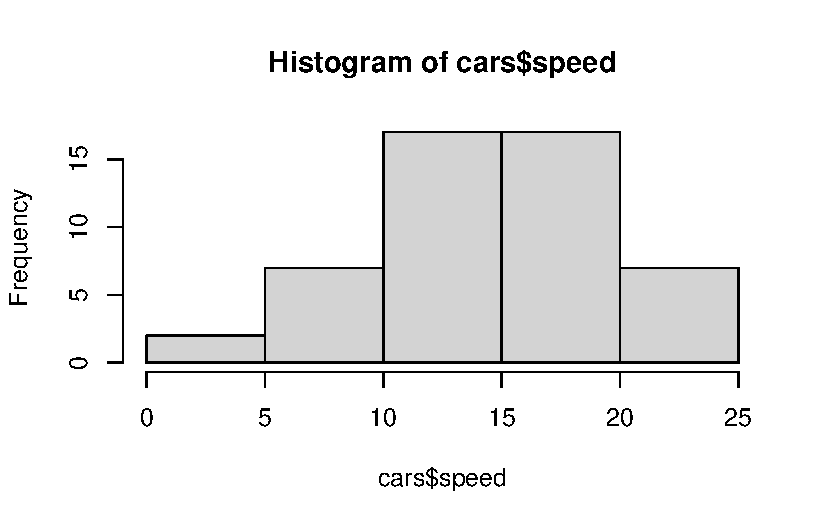
\includegraphics{summary_files/figure-pdf/unnamed-chunk-1-1.pdf}

\bookmarksetup{startatroot}

\chapter*{Література}\label{ux43bux456ux442ux435ux440ux430ux442ux443ux440ux430}
\addcontentsline{toc}{chapter}{Література}

\markboth{Література}{Література}

\phantomsection\label{refs}
\begin{CSLReferences}{0}{1}
\end{CSLReferences}



\end{document}
